
\newsavebox{\boxshapea}
\sbox{\boxshapea}{
  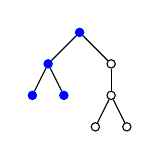
\begin{tikzpicture}[baseline=-0.5ex, scale=0.4]
    \tikzset{every node/.style={draw, circle, inner sep=0.5pt, minimum size=3pt}}
    \node[fill=Blue, draw=Blue] (ND) at (-1.62, -2) {};
    \node[fill=Blue, draw=Blue] (NE) at (-0.62, -2) {};
    \node[fill=Blue, draw=Blue] (NB) at (-1.12, -1) {};
    \node[] (NG) at (0.38, -3) {};
    \node[] (NH) at (1.38, -3) {};
    \node[] (NF) at (0.88, -2) {};
    \node[] (NC) at (0.88, -1) {};
    \node[fill=Blue, draw=Blue] (NA) at (-0.12, 0) {};
    \draw (NA) -- (NB);
    \draw (NB) -- (ND);
    \draw (NB) -- (NE);
    \draw (NA) -- (NC);
    \draw (NC) -- (NF);
    \draw (NF) -- (NG);
    \draw (NF) -- (NH);
  \end{tikzpicture}
}
\newsavebox{\boxshapeb}
\sbox{\boxshapeb}{
  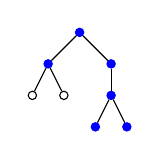
\begin{tikzpicture}[baseline=-0.5ex, scale=0.4]
    \tikzset{every node/.style={draw, circle, inner sep=0.5pt, minimum size=3pt}}
    \node[] (ND) at (-1.62, -2) {};
    \node[] (NE) at (-0.62, -2) {};
    \node[fill=Blue, draw=Blue] (NB) at (-1.12, -1) {};
    \node[fill=Blue, draw=Blue] (NG) at (0.38, -3) {};
    \node[fill=Blue, draw=Blue] (NH) at (1.38, -3) {};
    \node[fill=Blue, draw=Blue] (NF) at (0.88, -2) {};
    \node[fill=Blue, draw=Blue] (NC) at (0.88, -1) {};
    \node[fill=Blue, draw=Blue] (NA) at (-0.12, 0) {};
    \draw (NA) -- (NB);
    \draw (NB) -- (ND);
    \draw (NB) -- (NE);
    \draw (NA) -- (NC);
    \draw (NC) -- (NF);
    \draw (NF) -- (NG);
    \draw (NF) -- (NH);
  \end{tikzpicture}
}
\newsavebox{\boxshapec}
\sbox{\boxshapec}{
  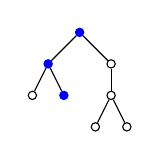
\begin{tikzpicture}[baseline=-0.5ex, scale=0.4]
    \tikzset{every node/.style={draw, circle, inner sep=0.5pt, minimum size=3pt}}
    \node[] (ND) at (-1.62, -2) {};
    \node[fill=Blue, draw=Blue] (NE) at (-0.62, -2) {};
    \node[fill=Blue, draw=Blue] (NB) at (-1.12, -1) {};
    \node[] (NG) at (0.38, -3) {};
    \node[] (NH) at (1.38, -3) {};
    \node[] (NF) at (0.88, -2) {};
    \node[] (NC) at (0.88, -1) {};
    \node[fill=Blue, draw=Blue] (NA) at (-0.12, 0) {};
    \draw (NA) -- (NB);
    \draw (NB) -- (ND);
    \draw (NB) -- (NE);
    \draw (NA) -- (NC);
    \draw (NC) -- (NF);
    \draw (NF) -- (NG);
    \draw (NF) -- (NH);
  \end{tikzpicture}
}
\newsavebox{\boxshaped}
\sbox{\boxshaped}{
  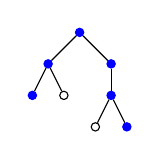
\begin{tikzpicture}[baseline=-0.5ex, scale=0.4]
    \tikzset{every node/.style={draw, circle, inner sep=0.5pt, minimum size=3pt}}
    \node[fill=Blue, draw=Blue] (ND) at (-1.62, -2) {};
    \node[] (NE) at (-0.62, -2) {};
    \node[fill=Blue, draw=Blue] (NB) at (-1.12, -1) {};
    \node[] (NG) at (0.38, -3) {};
    \node[fill=Blue, draw=Blue] (NH) at (1.38, -3) {};
    \node[fill=Blue, draw=Blue] (NF) at (0.88, -2) {};
    \node[fill=Blue, draw=Blue] (NC) at (0.88, -1) {};
    \node[fill=Blue, draw=Blue] (NA) at (-0.12, 0) {};
    \draw (NA) -- (NB);
    \draw (NB) -- (ND);
    \draw (NB) -- (NE);
    \draw (NA) -- (NC);
    \draw (NC) -- (NF);
    \draw (NF) -- (NG);
    \draw (NF) -- (NH);
  \end{tikzpicture}
}
\newsavebox{\boxshapee}
\sbox{\boxshapee}{
  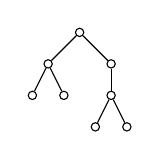
\begin{tikzpicture}[baseline=-0.5ex, scale=0.4]
    \tikzset{every node/.style={draw, circle, inner sep=0.5pt, minimum size=3pt}}
    \node[] (ND) at (-1.62, -2) {};
    \node[] (NE) at (-0.62, -2) {};
    \node[] (NB) at (-1.12, -1) {};
    \node[] (NG) at (0.38, -3) {};
    \node[] (NH) at (1.38, -3) {};
    \node[] (NF) at (0.88, -2) {};
    \node[] (NC) at (0.88, -1) {};
    \node[] (NA) at (-0.12, 0) {};
    \draw (NA) -- (NB);
    \draw (NB) -- (ND);
    \draw (NB) -- (NE);
    \draw (NA) -- (NC);
    \draw (NC) -- (NF);
    \draw (NF) -- (NG);
    \draw (NF) -- (NH);
  \end{tikzpicture}
}
\newsavebox{\boxshapef}
\sbox{\boxshapef}{
  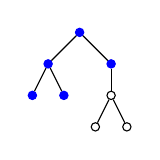
\begin{tikzpicture}[baseline=-0.5ex, scale=0.4]
    \tikzset{every node/.style={draw, circle, inner sep=0.5pt, minimum size=3pt}}
    \node[fill=Blue, draw=Blue] (ND) at (-1.62, -2) {};
    \node[fill=Blue, draw=Blue] (NE) at (-0.62, -2) {};
    \node[fill=Blue, draw=Blue] (NB) at (-1.12, -1) {};
    \node[] (NG) at (0.38, -3) {};
    \node[] (NH) at (1.38, -3) {};
    \node[] (NF) at (0.88, -2) {};
    \node[fill=Blue, draw=Blue] (NC) at (0.88, -1) {};
    \node[fill=Blue, draw=Blue] (NA) at (-0.12, 0) {};
    \draw (NA) -- (NB);
    \draw (NB) -- (ND);
    \draw (NB) -- (NE);
    \draw (NA) -- (NC);
    \draw (NC) -- (NF);
    \draw (NF) -- (NG);
    \draw (NF) -- (NH);
  \end{tikzpicture}
}
\newsavebox{\boxshapeg}
\sbox{\boxshapeg}{
  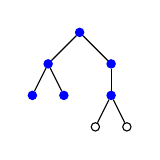
\begin{tikzpicture}[baseline=-0.5ex, scale=0.4]
    \tikzset{every node/.style={draw, circle, inner sep=0.5pt, minimum size=3pt}}
    \node[fill=Blue, draw=Blue] (ND) at (-1.62, -2) {};
    \node[fill=Blue, draw=Blue] (NE) at (-0.62, -2) {};
    \node[fill=Blue, draw=Blue] (NB) at (-1.12, -1) {};
    \node[] (NG) at (0.38, -3) {};
    \node[] (NH) at (1.38, -3) {};
    \node[fill=Blue, draw=Blue] (NF) at (0.88, -2) {};
    \node[fill=Blue, draw=Blue] (NC) at (0.88, -1) {};
    \node[fill=Blue, draw=Blue] (NA) at (-0.12, 0) {};
    \draw (NA) -- (NB);
    \draw (NB) -- (ND);
    \draw (NB) -- (NE);
    \draw (NA) -- (NC);
    \draw (NC) -- (NF);
    \draw (NF) -- (NG);
    \draw (NF) -- (NH);
  \end{tikzpicture}
}
\newsavebox{\boxshapeh}
\sbox{\boxshapeh}{
  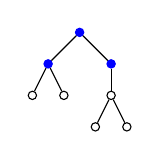
\begin{tikzpicture}[baseline=-0.5ex, scale=0.4]
    \tikzset{every node/.style={draw, circle, inner sep=0.5pt, minimum size=3pt}}
    \node[] (ND) at (-1.62, -2) {};
    \node[] (NE) at (-0.62, -2) {};
    \node[fill=Blue, draw=Blue] (NB) at (-1.12, -1) {};
    \node[] (NG) at (0.38, -3) {};
    \node[] (NH) at (1.38, -3) {};
    \node[] (NF) at (0.88, -2) {};
    \node[fill=Blue, draw=Blue] (NC) at (0.88, -1) {};
    \node[fill=Blue, draw=Blue] (NA) at (-0.12, 0) {};
    \draw (NA) -- (NB);
    \draw (NB) -- (ND);
    \draw (NB) -- (NE);
    \draw (NA) -- (NC);
    \draw (NC) -- (NF);
    \draw (NF) -- (NG);
    \draw (NF) -- (NH);
  \end{tikzpicture}
}
\newsavebox{\boxshapei}
\sbox{\boxshapei}{
  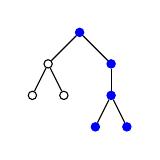
\begin{tikzpicture}[baseline=-0.5ex, scale=0.4]
    \tikzset{every node/.style={draw, circle, inner sep=0.5pt, minimum size=3pt}}
    \node[] (ND) at (-1.62, -2) {};
    \node[] (NE) at (-0.62, -2) {};
    \node[] (NB) at (-1.12, -1) {};
    \node[fill=Blue, draw=Blue] (NG) at (0.38, -3) {};
    \node[fill=Blue, draw=Blue] (NH) at (1.38, -3) {};
    \node[fill=Blue, draw=Blue] (NF) at (0.88, -2) {};
    \node[fill=Blue, draw=Blue] (NC) at (0.88, -1) {};
    \node[fill=Blue, draw=Blue] (NA) at (-0.12, 0) {};
    \draw (NA) -- (NB);
    \draw (NB) -- (ND);
    \draw (NB) -- (NE);
    \draw (NA) -- (NC);
    \draw (NC) -- (NF);
    \draw (NF) -- (NG);
    \draw (NF) -- (NH);
  \end{tikzpicture}
}
\newsavebox{\boxshapej}
\sbox{\boxshapej}{
  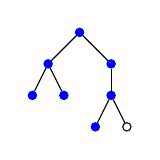
\begin{tikzpicture}[baseline=-0.5ex, scale=0.4]
    \tikzset{every node/.style={draw, circle, inner sep=0.5pt, minimum size=3pt}}
    \node[fill=Blue, draw=Blue] (ND) at (-1.62, -2) {};
    \node[fill=Blue, draw=Blue] (NE) at (-0.62, -2) {};
    \node[fill=Blue, draw=Blue] (NB) at (-1.12, -1) {};
    \node[fill=Blue, draw=Blue] (NG) at (0.38, -3) {};
    \node[] (NH) at (1.38, -3) {};
    \node[fill=Blue, draw=Blue] (NF) at (0.88, -2) {};
    \node[fill=Blue, draw=Blue] (NC) at (0.88, -1) {};
    \node[fill=Blue, draw=Blue] (NA) at (-0.12, 0) {};
    \draw (NA) -- (NB);
    \draw (NB) -- (ND);
    \draw (NB) -- (NE);
    \draw (NA) -- (NC);
    \draw (NC) -- (NF);
    \draw (NF) -- (NG);
    \draw (NF) -- (NH);
  \end{tikzpicture}
}
\newsavebox{\boxshapek}
\sbox{\boxshapek}{
  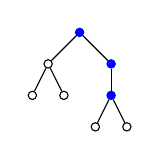
\begin{tikzpicture}[baseline=-0.5ex, scale=0.4]
    \tikzset{every node/.style={draw, circle, inner sep=0.5pt, minimum size=3pt}}
    \node[] (ND) at (-1.62, -2) {};
    \node[] (NE) at (-0.62, -2) {};
    \node[] (NB) at (-1.12, -1) {};
    \node[] (NG) at (0.38, -3) {};
    \node[] (NH) at (1.38, -3) {};
    \node[fill=Blue, draw=Blue] (NF) at (0.88, -2) {};
    \node[fill=Blue, draw=Blue] (NC) at (0.88, -1) {};
    \node[fill=Blue, draw=Blue] (NA) at (-0.12, 0) {};
    \draw (NA) -- (NB);
    \draw (NB) -- (ND);
    \draw (NB) -- (NE);
    \draw (NA) -- (NC);
    \draw (NC) -- (NF);
    \draw (NF) -- (NG);
    \draw (NF) -- (NH);
  \end{tikzpicture}
}
\newsavebox{\boxshapel}
\sbox{\boxshapel}{
  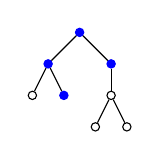
\begin{tikzpicture}[baseline=-0.5ex, scale=0.4]
    \tikzset{every node/.style={draw, circle, inner sep=0.5pt, minimum size=3pt}}
    \node[] (ND) at (-1.62, -2) {};
    \node[fill=Blue, draw=Blue] (NE) at (-0.62, -2) {};
    \node[fill=Blue, draw=Blue] (NB) at (-1.12, -1) {};
    \node[] (NG) at (0.38, -3) {};
    \node[] (NH) at (1.38, -3) {};
    \node[] (NF) at (0.88, -2) {};
    \node[fill=Blue, draw=Blue] (NC) at (0.88, -1) {};
    \node[fill=Blue, draw=Blue] (NA) at (-0.12, 0) {};
    \draw (NA) -- (NB);
    \draw (NB) -- (ND);
    \draw (NB) -- (NE);
    \draw (NA) -- (NC);
    \draw (NC) -- (NF);
    \draw (NF) -- (NG);
    \draw (NF) -- (NH);
  \end{tikzpicture}
}
\newsavebox{\boxshapem}
\sbox{\boxshapem}{
  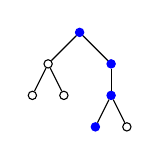
\begin{tikzpicture}[baseline=-0.5ex, scale=0.4]
    \tikzset{every node/.style={draw, circle, inner sep=0.5pt, minimum size=3pt}}
    \node[] (ND) at (-1.62, -2) {};
    \node[] (NE) at (-0.62, -2) {};
    \node[] (NB) at (-1.12, -1) {};
    \node[fill=Blue, draw=Blue] (NG) at (0.38, -3) {};
    \node[] (NH) at (1.38, -3) {};
    \node[fill=Blue, draw=Blue] (NF) at (0.88, -2) {};
    \node[fill=Blue, draw=Blue] (NC) at (0.88, -1) {};
    \node[fill=Blue, draw=Blue] (NA) at (-0.12, 0) {};
    \draw (NA) -- (NB);
    \draw (NB) -- (ND);
    \draw (NB) -- (NE);
    \draw (NA) -- (NC);
    \draw (NC) -- (NF);
    \draw (NF) -- (NG);
    \draw (NF) -- (NH);
  \end{tikzpicture}
}
\newsavebox{\boxshapen}
\sbox{\boxshapen}{
  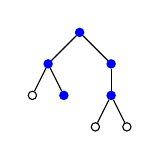
\begin{tikzpicture}[baseline=-0.5ex, scale=0.4]
    \tikzset{every node/.style={draw, circle, inner sep=0.5pt, minimum size=3pt}}
    \node[] (ND) at (-1.62, -2) {};
    \node[fill=Blue, draw=Blue] (NE) at (-0.62, -2) {};
    \node[fill=Blue, draw=Blue] (NB) at (-1.12, -1) {};
    \node[] (NG) at (0.38, -3) {};
    \node[] (NH) at (1.38, -3) {};
    \node[fill=Blue, draw=Blue] (NF) at (0.88, -2) {};
    \node[fill=Blue, draw=Blue] (NC) at (0.88, -1) {};
    \node[fill=Blue, draw=Blue] (NA) at (-0.12, 0) {};
    \draw (NA) -- (NB);
    \draw (NB) -- (ND);
    \draw (NB) -- (NE);
    \draw (NA) -- (NC);
    \draw (NC) -- (NF);
    \draw (NF) -- (NG);
    \draw (NF) -- (NH);
  \end{tikzpicture}
}
\newsavebox{\boxshapeo}
\sbox{\boxshapeo}{
  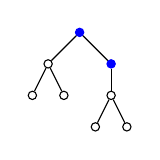
\begin{tikzpicture}[baseline=-0.5ex, scale=0.4]
    \tikzset{every node/.style={draw, circle, inner sep=0.5pt, minimum size=3pt}}
    \node[] (ND) at (-1.62, -2) {};
    \node[] (NE) at (-0.62, -2) {};
    \node[] (NB) at (-1.12, -1) {};
    \node[] (NG) at (0.38, -3) {};
    \node[] (NH) at (1.38, -3) {};
    \node[] (NF) at (0.88, -2) {};
    \node[fill=Blue, draw=Blue] (NC) at (0.88, -1) {};
    \node[fill=Blue, draw=Blue] (NA) at (-0.12, 0) {};
    \draw (NA) -- (NB);
    \draw (NB) -- (ND);
    \draw (NB) -- (NE);
    \draw (NA) -- (NC);
    \draw (NC) -- (NF);
    \draw (NF) -- (NG);
    \draw (NF) -- (NH);
  \end{tikzpicture}
}
\newsavebox{\boxshapep}
\sbox{\boxshapep}{
  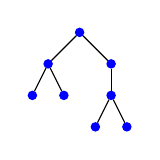
\begin{tikzpicture}[baseline=-0.5ex, scale=0.4]
    \tikzset{every node/.style={draw, circle, inner sep=0.5pt, minimum size=3pt}}
    \node[fill=Blue, draw=Blue] (ND) at (-1.62, -2) {};
    \node[fill=Blue, draw=Blue] (NE) at (-0.62, -2) {};
    \node[fill=Blue, draw=Blue] (NB) at (-1.12, -1) {};
    \node[fill=Blue, draw=Blue] (NG) at (0.38, -3) {};
    \node[fill=Blue, draw=Blue] (NH) at (1.38, -3) {};
    \node[fill=Blue, draw=Blue] (NF) at (0.88, -2) {};
    \node[fill=Blue, draw=Blue] (NC) at (0.88, -1) {};
    \node[fill=Blue, draw=Blue] (NA) at (-0.12, 0) {};
    \draw (NA) -- (NB);
    \draw (NB) -- (ND);
    \draw (NB) -- (NE);
    \draw (NA) -- (NC);
    \draw (NC) -- (NF);
    \draw (NF) -- (NG);
    \draw (NF) -- (NH);
  \end{tikzpicture}
}
\newsavebox{\boxshapeq}
\sbox{\boxshapeq}{
  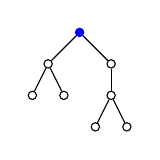
\begin{tikzpicture}[baseline=-0.5ex, scale=0.4]
    \tikzset{every node/.style={draw, circle, inner sep=0.5pt, minimum size=3pt}}
    \node[] (ND) at (-1.62, -2) {};
    \node[] (NE) at (-0.62, -2) {};
    \node[] (NB) at (-1.12, -1) {};
    \node[] (NG) at (0.38, -3) {};
    \node[] (NH) at (1.38, -3) {};
    \node[] (NF) at (0.88, -2) {};
    \node[] (NC) at (0.88, -1) {};
    \node[fill=Blue, draw=Blue] (NA) at (-0.12, 0) {};
    \draw (NA) -- (NB);
    \draw (NB) -- (ND);
    \draw (NB) -- (NE);
    \draw (NA) -- (NC);
    \draw (NC) -- (NF);
    \draw (NF) -- (NG);
    \draw (NF) -- (NH);
  \end{tikzpicture}
}
\newsavebox{\boxshaper}
\sbox{\boxshaper}{
  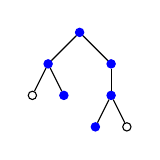
\begin{tikzpicture}[baseline=-0.5ex, scale=0.4]
    \tikzset{every node/.style={draw, circle, inner sep=0.5pt, minimum size=3pt}}
    \node[] (ND) at (-1.62, -2) {};
    \node[fill=Blue, draw=Blue] (NE) at (-0.62, -2) {};
    \node[fill=Blue, draw=Blue] (NB) at (-1.12, -1) {};
    \node[fill=Blue, draw=Blue] (NG) at (0.38, -3) {};
    \node[] (NH) at (1.38, -3) {};
    \node[fill=Blue, draw=Blue] (NF) at (0.88, -2) {};
    \node[fill=Blue, draw=Blue] (NC) at (0.88, -1) {};
    \node[fill=Blue, draw=Blue] (NA) at (-0.12, 0) {};
    \draw (NA) -- (NB);
    \draw (NB) -- (ND);
    \draw (NB) -- (NE);
    \draw (NA) -- (NC);
    \draw (NC) -- (NF);
    \draw (NF) -- (NG);
    \draw (NF) -- (NH);
  \end{tikzpicture}
}
\providecommand{\boxshapes}{\newsavebox{\boxshapes}}
\sbox{\boxshapes}{
  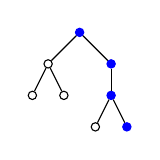
\begin{tikzpicture}[baseline=-0.5ex, scale=0.4]
    \tikzset{every node/.style={draw, circle, inner sep=0.5pt, minimum size=3pt}}
    \node[] (ND) at (-1.62, -2) {};
    \node[] (NE) at (-0.62, -2) {};
    \node[] (NB) at (-1.12, -1) {};
    \node[] (NG) at (0.38, -3) {};
    \node[fill=Blue, draw=Blue] (NH) at (1.38, -3) {};
    \node[fill=Blue, draw=Blue] (NF) at (0.88, -2) {};
    \node[fill=Blue, draw=Blue] (NC) at (0.88, -1) {};
    \node[fill=Blue, draw=Blue] (NA) at (-0.12, 0) {};
    \draw (NA) -- (NB);
    \draw (NB) -- (ND);
    \draw (NB) -- (NE);
    \draw (NA) -- (NC);
    \draw (NC) -- (NF);
    \draw (NF) -- (NG);
    \draw (NF) -- (NH);
  \end{tikzpicture}
}
\newsavebox{\boxshapet}
\sbox{\boxshapet}{
  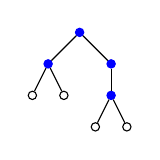
\begin{tikzpicture}[baseline=-0.5ex, scale=0.4]
    \tikzset{every node/.style={draw, circle, inner sep=0.5pt, minimum size=3pt}}
    \node[] (ND) at (-1.62, -2) {};
    \node[] (NE) at (-0.62, -2) {};
    \node[fill=Blue, draw=Blue] (NB) at (-1.12, -1) {};
    \node[] (NG) at (0.38, -3) {};
    \node[] (NH) at (1.38, -3) {};
    \node[fill=Blue, draw=Blue] (NF) at (0.88, -2) {};
    \node[fill=Blue, draw=Blue] (NC) at (0.88, -1) {};
    \node[fill=Blue, draw=Blue] (NA) at (-0.12, 0) {};
    \draw (NA) -- (NB);
    \draw (NB) -- (ND);
    \draw (NB) -- (NE);
    \draw (NA) -- (NC);
    \draw (NC) -- (NF);
    \draw (NF) -- (NG);
    \draw (NF) -- (NH);
  \end{tikzpicture}
}
\newsavebox{\boxshapeu}
\sbox{\boxshapeu}{
  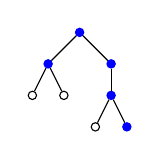
\begin{tikzpicture}[baseline=-0.5ex, scale=0.4]
    \tikzset{every node/.style={draw, circle, inner sep=0.5pt, minimum size=3pt}}
    \node[] (ND) at (-1.62, -2) {};
    \node[] (NE) at (-0.62, -2) {};
    \node[fill=Blue, draw=Blue] (NB) at (-1.12, -1) {};
    \node[] (NG) at (0.38, -3) {};
    \node[fill=Blue, draw=Blue] (NH) at (1.38, -3) {};
    \node[fill=Blue, draw=Blue] (NF) at (0.88, -2) {};
    \node[fill=Blue, draw=Blue] (NC) at (0.88, -1) {};
    \node[fill=Blue, draw=Blue] (NA) at (-0.12, 0) {};
    \draw (NA) -- (NB);
    \draw (NB) -- (ND);
    \draw (NB) -- (NE);
    \draw (NA) -- (NC);
    \draw (NC) -- (NF);
    \draw (NF) -- (NG);
    \draw (NF) -- (NH);
  \end{tikzpicture}
}
\newsavebox{\boxshapev}
\sbox{\boxshapev}{
  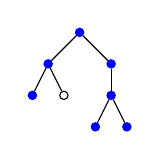
\begin{tikzpicture}[baseline=-0.5ex, scale=0.4]
    \tikzset{every node/.style={draw, circle, inner sep=0.5pt, minimum size=3pt}}
    \node[fill=Blue, draw=Blue] (ND) at (-1.62, -2) {};
    \node[] (NE) at (-0.62, -2) {};
    \node[fill=Blue, draw=Blue] (NB) at (-1.12, -1) {};
    \node[fill=Blue, draw=Blue] (NG) at (0.38, -3) {};
    \node[fill=Blue, draw=Blue] (NH) at (1.38, -3) {};
    \node[fill=Blue, draw=Blue] (NF) at (0.88, -2) {};
    \node[fill=Blue, draw=Blue] (NC) at (0.88, -1) {};
    \node[fill=Blue, draw=Blue] (NA) at (-0.12, 0) {};
    \draw (NA) -- (NB);
    \draw (NB) -- (ND);
    \draw (NB) -- (NE);
    \draw (NA) -- (NC);
    \draw (NC) -- (NF);
    \draw (NF) -- (NG);
    \draw (NF) -- (NH);
  \end{tikzpicture}
}
\newsavebox{\boxshapew}
\sbox{\boxshapew}{
  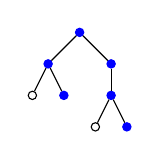
\begin{tikzpicture}[baseline=-0.5ex, scale=0.4]
    \tikzset{every node/.style={draw, circle, inner sep=0.5pt, minimum size=3pt}}
    \node[] (ND) at (-1.62, -2) {};
    \node[fill=Blue, draw=Blue] (NE) at (-0.62, -2) {};
    \node[fill=Blue, draw=Blue] (NB) at (-1.12, -1) {};
    \node[] (NG) at (0.38, -3) {};
    \node[fill=Blue, draw=Blue] (NH) at (1.38, -3) {};
    \node[fill=Blue, draw=Blue] (NF) at (0.88, -2) {};
    \node[fill=Blue, draw=Blue] (NC) at (0.88, -1) {};
    \node[fill=Blue, draw=Blue] (NA) at (-0.12, 0) {};
    \draw (NA) -- (NB);
    \draw (NB) -- (ND);
    \draw (NB) -- (NE);
    \draw (NA) -- (NC);
    \draw (NC) -- (NF);
    \draw (NF) -- (NG);
    \draw (NF) -- (NH);
  \end{tikzpicture}
}
\newsavebox{\boxshapex}
\sbox{\boxshapex}{
  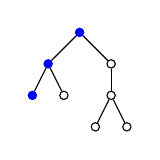
\begin{tikzpicture}[baseline=-0.5ex, scale=0.4]
    \tikzset{every node/.style={draw, circle, inner sep=0.5pt, minimum size=3pt}}
    \node[fill=Blue, draw=Blue] (ND) at (-1.62, -2) {};
    \node[] (NE) at (-0.62, -2) {};
    \node[fill=Blue, draw=Blue] (NB) at (-1.12, -1) {};
    \node[] (NG) at (0.38, -3) {};
    \node[] (NH) at (1.38, -3) {};
    \node[] (NF) at (0.88, -2) {};
    \node[] (NC) at (0.88, -1) {};
    \node[fill=Blue, draw=Blue] (NA) at (-0.12, 0) {};
    \draw (NA) -- (NB);
    \draw (NB) -- (ND);
    \draw (NB) -- (NE);
    \draw (NA) -- (NC);
    \draw (NC) -- (NF);
    \draw (NF) -- (NG);
    \draw (NF) -- (NH);
  \end{tikzpicture}
}
\newsavebox{\boxshapey}
\sbox{\boxshapey}{
  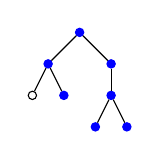
\begin{tikzpicture}[baseline=-0.5ex, scale=0.4]
    \tikzset{every node/.style={draw, circle, inner sep=0.5pt, minimum size=3pt}}
    \node[] (ND) at (-1.62, -2) {};
    \node[fill=Blue, draw=Blue] (NE) at (-0.62, -2) {};
    \node[fill=Blue, draw=Blue] (NB) at (-1.12, -1) {};
    \node[fill=Blue, draw=Blue] (NG) at (0.38, -3) {};
    \node[fill=Blue, draw=Blue] (NH) at (1.38, -3) {};
    \node[fill=Blue, draw=Blue] (NF) at (0.88, -2) {};
    \node[fill=Blue, draw=Blue] (NC) at (0.88, -1) {};
    \node[fill=Blue, draw=Blue] (NA) at (-0.12, 0) {};
    \draw (NA) -- (NB);
    \draw (NB) -- (ND);
    \draw (NB) -- (NE);
    \draw (NA) -- (NC);
    \draw (NC) -- (NF);
    \draw (NF) -- (NG);
    \draw (NF) -- (NH);
  \end{tikzpicture}
}
\newsavebox{\boxshapez}
\sbox{\boxshapez}{
  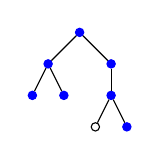
\begin{tikzpicture}[baseline=-0.5ex, scale=0.4]
    \tikzset{every node/.style={draw, circle, inner sep=0.5pt, minimum size=3pt}}
    \node[fill=Blue, draw=Blue] (ND) at (-1.62, -2) {};
    \node[fill=Blue, draw=Blue] (NE) at (-0.62, -2) {};
    \node[fill=Blue, draw=Blue] (NB) at (-1.12, -1) {};
    \node[] (NG) at (0.38, -3) {};
    \node[fill=Blue, draw=Blue] (NH) at (1.38, -3) {};
    \node[fill=Blue, draw=Blue] (NF) at (0.88, -2) {};
    \node[fill=Blue, draw=Blue] (NC) at (0.88, -1) {};
    \node[fill=Blue, draw=Blue] (NA) at (-0.12, 0) {};
    \draw (NA) -- (NB);
    \draw (NB) -- (ND);
    \draw (NB) -- (NE);
    \draw (NA) -- (NC);
    \draw (NC) -- (NF);
    \draw (NF) -- (NG);
    \draw (NF) -- (NH);
  \end{tikzpicture}
}
\newsavebox{\boxshapeaa}
\sbox{\boxshapeaa}{
  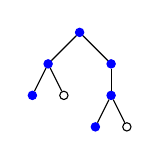
\begin{tikzpicture}[baseline=-0.5ex, scale=0.4]
    \tikzset{every node/.style={draw, circle, inner sep=0.5pt, minimum size=3pt}}
    \node[fill=Blue, draw=Blue] (ND) at (-1.62, -2) {};
    \node[] (NE) at (-0.62, -2) {};
    \node[fill=Blue, draw=Blue] (NB) at (-1.12, -1) {};
    \node[fill=Blue, draw=Blue] (NG) at (0.38, -3) {};
    \node[] (NH) at (1.38, -3) {};
    \node[fill=Blue, draw=Blue] (NF) at (0.88, -2) {};
    \node[fill=Blue, draw=Blue] (NC) at (0.88, -1) {};
    \node[fill=Blue, draw=Blue] (NA) at (-0.12, 0) {};
    \draw (NA) -- (NB);
    \draw (NB) -- (ND);
    \draw (NB) -- (NE);
    \draw (NA) -- (NC);
    \draw (NC) -- (NF);
    \draw (NF) -- (NG);
    \draw (NF) -- (NH);
  \end{tikzpicture}
}
\newsavebox{\boxshapeab}
\sbox{\boxshapeab}{
  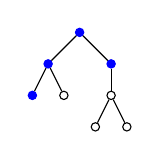
\begin{tikzpicture}[baseline=-0.5ex, scale=0.4]
    \tikzset{every node/.style={draw, circle, inner sep=0.5pt, minimum size=3pt}}
    \node[fill=Blue, draw=Blue] (ND) at (-1.62, -2) {};
    \node[] (NE) at (-0.62, -2) {};
    \node[fill=Blue, draw=Blue] (NB) at (-1.12, -1) {};
    \node[] (NG) at (0.38, -3) {};
    \node[] (NH) at (1.38, -3) {};
    \node[] (NF) at (0.88, -2) {};
    \node[fill=Blue, draw=Blue] (NC) at (0.88, -1) {};
    \node[fill=Blue, draw=Blue] (NA) at (-0.12, 0) {};
    \draw (NA) -- (NB);
    \draw (NB) -- (ND);
    \draw (NB) -- (NE);
    \draw (NA) -- (NC);
    \draw (NC) -- (NF);
    \draw (NF) -- (NG);
    \draw (NF) -- (NH);
  \end{tikzpicture}
}
\newsavebox{\boxshapeac}
\sbox{\boxshapeac}{
  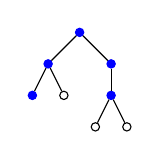
\begin{tikzpicture}[baseline=-0.5ex, scale=0.4]
    \tikzset{every node/.style={draw, circle, inner sep=0.5pt, minimum size=3pt}}
    \node[fill=Blue, draw=Blue] (ND) at (-1.62, -2) {};
    \node[] (NE) at (-0.62, -2) {};
    \node[fill=Blue, draw=Blue] (NB) at (-1.12, -1) {};
    \node[] (NG) at (0.38, -3) {};
    \node[] (NH) at (1.38, -3) {};
    \node[fill=Blue, draw=Blue] (NF) at (0.88, -2) {};
    \node[fill=Blue, draw=Blue] (NC) at (0.88, -1) {};
    \node[fill=Blue, draw=Blue] (NA) at (-0.12, 0) {};
    \draw (NA) -- (NB);
    \draw (NB) -- (ND);
    \draw (NB) -- (NE);
    \draw (NA) -- (NC);
    \draw (NC) -- (NF);
    \draw (NF) -- (NG);
    \draw (NF) -- (NH);
  \end{tikzpicture}
}
\newsavebox{\boxshapead}
\sbox{\boxshapead}{
  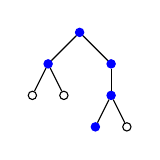
\begin{tikzpicture}[baseline=-0.5ex, scale=0.4]
    \tikzset{every node/.style={draw, circle, inner sep=0.5pt, minimum size=3pt}}
    \node[] (ND) at (-1.62, -2) {};
    \node[] (NE) at (-0.62, -2) {};
    \node[fill=Blue, draw=Blue] (NB) at (-1.12, -1) {};
    \node[fill=Blue, draw=Blue] (NG) at (0.38, -3) {};
    \node[] (NH) at (1.38, -3) {};
    \node[fill=Blue, draw=Blue] (NF) at (0.88, -2) {};
    \node[fill=Blue, draw=Blue] (NC) at (0.88, -1) {};
    \node[fill=Blue, draw=Blue] (NA) at (-0.12, 0) {};
    \draw (NA) -- (NB);
    \draw (NB) -- (ND);
    \draw (NB) -- (NE);
    \draw (NA) -- (NC);
    \draw (NC) -- (NF);
    \draw (NF) -- (NG);
    \draw (NF) -- (NH);
  \end{tikzpicture}
}
\newsavebox{\boxshapeae}
\sbox{\boxshapeae}{
  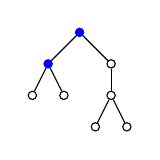
\begin{tikzpicture}[baseline=-0.5ex, scale=0.4]
    \tikzset{every node/.style={draw, circle, inner sep=0.5pt, minimum size=3pt}}
    \node[] (ND) at (-1.62, -2) {};
    \node[] (NE) at (-0.62, -2) {};
    \node[fill=Blue, draw=Blue] (NB) at (-1.12, -1) {};
    \node[] (NG) at (0.38, -3) {};
    \node[] (NH) at (1.38, -3) {};
    \node[] (NF) at (0.88, -2) {};
    \node[] (NC) at (0.88, -1) {};
    \node[fill=Blue, draw=Blue] (NA) at (-0.12, 0) {};
    \draw (NA) -- (NB);
    \draw (NB) -- (ND);
    \draw (NB) -- (NE);
    \draw (NA) -- (NC);
    \draw (NC) -- (NF);
    \draw (NF) -- (NG);
    \draw (NF) -- (NH);
  \end{tikzpicture}
}
\begin{tikzpicture}[xscale=2.8, yscale=1.8]
\newcommand{\edgespathclr}{Blue}
\newcommand{\edgesclr}{gray}
\coordinate (A-B-D-E) at (3.20, 4);
\coordinate (A-B-C-F-G-H) at (0.00, 6);
\coordinate (A-B-E) at (2.67, 3);
\coordinate (A-B-C-D-F-H) at (3.20, 6);
\coordinate (empty) at (2.00, 0);
\coordinate (A-B-C-D-E) at (3.20, 5);
\coordinate (A-B-C-D-E-F) at (2.40, 6);
\coordinate (A-B-C) at (1.33, 3);
\coordinate (A-C-F-G-H) at (0.00, 5);
\coordinate (A-B-C-D-E-F-G) at (1.33, 7);
\coordinate (A-C-F) at (0.00, 3);
\coordinate (A-B-C-E) at (2.40, 4);
\coordinate (A-C-F-G) at (0.80, 4);
\coordinate (A-B-C-E-F) at (2.40, 5);
\coordinate (A-C) at (0.00, 2);
\coordinate (A-B-C-D-E-F-G-H) at (2.00, 8);
\coordinate (A) at (2.00, 1);
\coordinate (A-B-C-E-F-G) at (1.60, 6);
\coordinate (A-C-F-H) at (0.00, 4);
\coordinate (A-B-C-F) at (1.60, 4);
\coordinate (A-B-C-F-H) at (1.60, 5);
\coordinate (A-B-C-D-F-G-H) at (4.00, 7);
\coordinate (A-B-C-E-F-H) at (0.80, 6);
\coordinate (A-B-D) at (4.00, 3);
\coordinate (A-B-C-E-F-G-H) at (0.00, 7);
\coordinate (A-B-C-D-E-F-H) at (2.67, 7);
\coordinate (A-B-C-D-F-G) at (4.00, 6);
\coordinate (A-B-C-D) at (4.00, 4);
\coordinate (A-B-C-D-F) at (4.00, 5);
\coordinate (A-B-C-F-G) at (0.80, 5);
\coordinate (A-B) at (4.00, 2);
\foreach\a/\b in {
A-B-C-D-F-H/A-B-C-D-E-F-H, A-B-C-D-F/A-B-C-D-F-G, A-B-C-F/A-B-C-E-F, A-B-C-F-G-H/A-B-C-E-F-G-H, A-B-C-F/A-B-C-F-G, A-B-C-E-F/A-B-C-E-F-G, A-B-C-E/A-B-C-D-E, A-B-E/A-B-D-E, A/A-B, A-B-C-D-F-G/A-B-C-D-F-G-H, A-B-C-D-F-G-H/A-B-C-D-E-F-G-H, A-B-C/A-B-C-F, A-B-C-D-E-F/A-B-C-D-E-F-H, A-C/A-B-C, A-B-C-F/A-B-C-F-H, A-B-C/A-B-C-E, A-B-C-D-E-F/A-B-C-D-E-F-G, A-B-C-D/A-B-C-D-E, A-B-C-D-E/A-B-C-D-E-F, A-B-C-D-F/A-B-C-D-E-F, A-B-D-E/A-B-C-D-E, A-C-F/A-C-F-G, A-C-F-G-H/A-B-C-F-G-H, A-B-C-E-F-G/A-B-C-E-F-G-H, A-B-C-D-E-F-H/A-B-C-D-E-F-G-H, A-B-D/A-B-D-E, A-B-C-E-F/A-B-C-D-E-F, A-B-C-F-H/A-B-C-E-F-H, A-B-C-E-F-G-H/A-B-C-D-E-F-G-H, A-C-F/A-B-C-F, A-B-C-F-H/A-B-C-F-G-H, A-B/A-B-C, A-C-F-G/A-C-F-G-H}{
    \draw[\edgesclr] (\a) -- (\b);
}
\draw[\edgesclr] (A-B) -- (A-B-D);
\foreach\a/\b in {
A-B-D/A-B-C-D, empty/A, A-B/A-B-E, A-B-C-D-E-F-H/A-B-C-D-E-F, A-C-F-G-H/A-C-F-G, A-B-C-D-F-G-H/A-B-C-D-F-G, A-B-C-E-F-H/A-B-C-E-F-G-H, A-B-C-F/A-B-C, A-B-E/A-B-C-E, A-B-C-D-E-F/A-B-C-D-E, A-B-C-E/A-B-C-E-F, A-B-C-D-E/A-B-D-E, A-B-D-E/A-B-D, A-B-C-D/A-B-C-D-F, A-C-F/A-C-F-H, A-B-C-E-F-G-H/A-B-C-E-F-G, A-B-C-F-H/A-B-C-F, A-B-C-F-G-H/A-B-C-F-H, A-C-F-H/A-C-F-G-H, A-B-C-D-E-F-G/A-B-C-D-E-F-G-H, A-B-C-E-F-G/A-B-C-D-E-F-G, A-B-C-D-F-H/A-B-C-D-F-G-H, A/A-C, A-B-C/A-B, A-B-C-F-G/A-B-C-F-G-H, A-B-C-D-E-F-G-H/A-B-C-D-E-F-H, A-C-F-G/A-B-C-F-G, A-B-C-E-F/A-B-C-E-F-H, A-B-C-D-F/A-B-C-D-F-H, A-C/A-C-F}{
    \draw[\edgespathclr, ultra thick] (\a) -- (\b);
}
\node[draw, fill=white, inner sep=2pt, rounded corners=2pt] at (A-B-D-E) {\usebox{\boxshapea}};
\node[draw, fill=white, inner sep=2pt, rounded corners=2pt] at (A-B-C-F-G-H) {\usebox{\boxshapeb}};
\node[draw, fill=white, inner sep=2pt, rounded corners=2pt] at (A-B-E) {\usebox{\boxshapec}};
\node[draw, fill=white, inner sep=2pt, rounded corners=2pt] at (A-B-C-D-F-H) {\usebox{\boxshaped}};
\node[draw, fill=white, inner sep=2pt, rounded corners=2pt] at (empty) {\usebox{\boxshapee}};
\node[draw, fill=white, inner sep=2pt, rounded corners=2pt] at (A-B-C-D-E) {\usebox{\boxshapef}};
\node[draw, fill=white, inner sep=2pt, rounded corners=2pt] at (A-B-C-D-E-F) {\usebox{\boxshapeg}};
\node[draw, fill=white, inner sep=2pt, rounded corners=2pt] at (A-B-C) {\usebox{\boxshapeh}};
\node[draw, fill=white, inner sep=2pt, rounded corners=2pt] at (A-C-F-G-H) {\usebox{\boxshapei}};
\node[draw, fill=white, inner sep=2pt, rounded corners=2pt] at (A-B-C-D-E-F-G) {\usebox{\boxshapej}};
\node[draw, fill=white, inner sep=2pt, rounded corners=2pt] at (A-C-F) {\usebox{\boxshapek}};
\node[draw, fill=white, inner sep=2pt, rounded corners=2pt] at (A-B-C-E) {\usebox{\boxshapel}};
\node[draw, fill=white, inner sep=2pt, rounded corners=2pt] at (A-C-F-G) {\usebox{\boxshapem}};
\node[draw, fill=white, inner sep=2pt, rounded corners=2pt] at (A-B-C-E-F) {\usebox{\boxshapen}};
\node[draw, fill=white, inner sep=2pt, rounded corners=2pt] at (A-C) {\usebox{\boxshapeo}};
\node[draw, fill=white, inner sep=2pt, rounded corners=2pt] at (A-B-C-D-E-F-G-H) {\usebox{\boxshapep}};
\node[draw, fill=white, inner sep=2pt, rounded corners=2pt] at (A) {\usebox{\boxshapeq}};
\node[draw, fill=white, inner sep=2pt, rounded corners=2pt] at (A-B-C-E-F-G) {\usebox{\boxshaper}};
\node[draw, fill=white, inner sep=2pt, rounded corners=2pt] at (A-C-F-H) {\usebox{\boxshapes}};
\node[draw, fill=white, inner sep=2pt, rounded corners=2pt] at (A-B-C-F) {\usebox{\boxshapet}};
\node[draw, fill=white, inner sep=2pt, rounded corners=2pt] at (A-B-C-F-H) {\usebox{\boxshapeu}};
\node[draw, fill=white, inner sep=2pt, rounded corners=2pt] at (A-B-C-D-F-G-H) {\usebox{\boxshapev}};
\node[draw, fill=white, inner sep=2pt, rounded corners=2pt] at (A-B-C-E-F-H) {\usebox{\boxshapew}};
\node[draw, fill=white, inner sep=2pt, rounded corners=2pt] at (A-B-D) {\usebox{\boxshapex}};
\node[draw, fill=white, inner sep=2pt, rounded corners=2pt] at (A-B-C-E-F-G-H) {\usebox{\boxshapey}};
\node[draw, fill=white, inner sep=2pt, rounded corners=2pt] at (A-B-C-D-E-F-H) {\usebox{\boxshapez}};
\node[draw, fill=white, inner sep=2pt, rounded corners=2pt] at (A-B-C-D-F-G) {\usebox{\boxshapeaa}};
\node[draw, fill=white, inner sep=2pt, rounded corners=2pt] at (A-B-C-D) {\usebox{\boxshapeab}};
\node[draw, fill=white, inner sep=2pt, rounded corners=2pt] at (A-B-C-D-F) {\usebox{\boxshapeac}};
\node[draw, fill=white, inner sep=2pt, rounded corners=2pt] at (A-B-C-F-G) {\usebox{\boxshapead}};
\node[draw, fill=white, inner sep=2pt, rounded corners=2pt] at (A-B) {\usebox{\boxshapeae}};
\end{tikzpicture}
